% !TeX root = ../main.tex

\subsection*{(k)PCA}

Our known approch is the principle component analysis (PCA).

\begin{figure}[H]
	\centering
	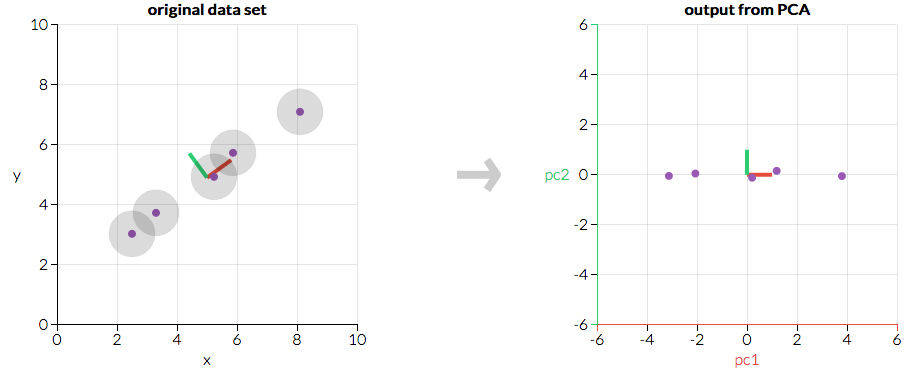
\includegraphics[width=0.8\textwidth]{pca}
\end{figure}

Orthogonal basis that is aligned with the ``maximum spread'' (w.r.t. the covariance) of the data. It is a global unsupervised method\footnote{Operating on all data points, no labels, find one global optimal solution}. Consider that PCA os a linear method.

\begin{figure}[H]
	\centering
	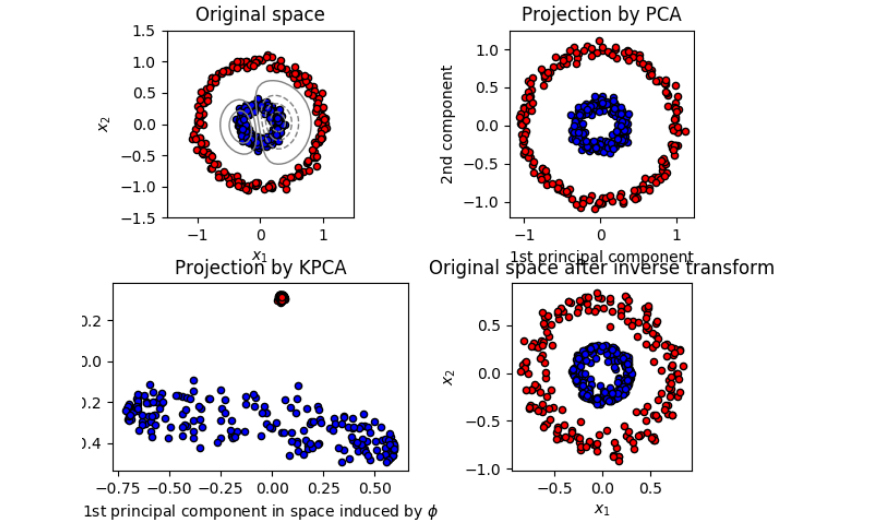
\includegraphics[width=0.7\textwidth]{k_pca}
\end{figure}

The Kernel PCA performs a non-linear mapping of the data, then perform a standard (linear) PCA on the result. With the kernel-trick we can do that in one step. The Objective function: (the non-linear mapping is part of $\phi$)

\begin{equation*}
    \delta = \sum_{i,j=1}^{N} (\phi(\vec{x_i}) - \phi(\vec{x_j}))^T (\phi(\vec{x_i}) - \phi(\vec{x_j})) + \lambda (\phi^T\phi-1)
\end{equation*}

Some offsprings of the Kernel PCA idea are:
\begin{enumerate}
    \item Perform some preprocessing / mapping that operates non-linearly
    \item The dimensionality reduction itself is an operation that operates linearly.
\end{enumerate}
